\chapter{Avaliação dos Modelos de Aprendizado de Máquina (AM)}

Este capítulo apresenta os resultados obtidos a partir da aplicação dos modelos de Aprendizado de Máquina desenvolvidos neste trabalho. 
Inicialmente, são discutidas as métricas de desempenho alcançadas pelos modelos na tarefa de predição da pontuação final das equipes. 
Em seguida, é realizada uma análise do comportamento das previsões, buscando avaliar a capacidade dos modelos em capturar padrões relevantes a partir das estatísticas 
individuais dos jogadores.

\section{Modelos de Aprendizado de Máquina (AM)}

O melhor modelo de AM desenvolvido neste estudo apresentou acurácia máxima de aproximadamente $55\%$ na tarefa de prever a pontuação final de um time em sua liga nacional, utilizando
como base os dados estatísticos de desempenho individual de seus jogadores na temporada anterior.

Para avaliar o desempenho dos diferentes algoritmos aplicados à tarefa de previsão, foram calculadas métricas 
amplamente utilizadas em problemas de regressão, incluindo o coeficiente de determinação (R\textsuperscript{2}), 
o erro absoluto médio (MAE), o erro quadrático médio (MSE), a raiz do erro quadrático médio (RMSE), 
o erro percentual absoluto médio (MAPE) e o tempo de processamento de cada modelo. A Tabela~\ref{tab:comparacao_modelos} 
apresenta um resumo comparativo dos resultados obtidos, permitindo analisar tanto a qualidade preditiva 
quanto o custo computacional de cada abordagem.

\begin{table}[H]
\centering
\caption{Comparação de desempenho entre os modelos de Machine Learning avaliados no conjunto de testes}
\label{tab:comparacao_modelos}
\begin{tabular}{lcccccc}
\hline
\textbf{Modelo} & \textbf{R\textsuperscript{2}} & \textbf{MAE} & \textbf{MSE} & \textbf{RMSE} & \textbf{MAPE} & \textbf{Tempo (s)} \\
\hline
RL      & 0.41 & 11.48 & 191.78 & 13.85 & 0.2580 & 2.15 \\
RF      & 0.28 & 12.05 & 234.05 & 15.30 & 0.2690 & 423.13 \\
XGBoost & 0.41 & 11.48 & 191.78 & 13.85 & 0.2580 & 2.86 \\
MLP     & 0.55 & 11.08 & 170.42 & 13.05 & 0.2424 & 161.68 \\
\hline
\end{tabular}

\vspace{0.3cm}
{\footnotesize \textit{Fonte:} Elaborado pelo autor.}

\end{table}

Os resultados apresentados na Tabela~\ref{tab:comparacao_modelos} evidenciam um comportamento consistente entre os algoritmos avaliados, com desempenho
moderado na tarefa de previsão da pontuação final dos times. Embora a acurácia máxima tenha alcançado aproximadamente $55\%$, observa-se que todos os modelos
enfrentam limitações inerentes à natureza imprevisível, ruidosa e não linear do problema. A pontuação de um time ao longo de uma temporada é influenciada também
por fatores não refletidos nas estatísticas individuais de jogadores, como variações táticas, mudanças de treinador, lesões, contexto competitivo e dinâmica
coletiva, o que naturalmente reduz o teto preditivo esperável.

Entre as abordagens testadas, a Rede Neural Multicamadas (MLP) apresentou o melhor equilíbrio entre qualidade preditiva e estabilidade, alcançando o maior valor de
R\textsuperscript{2} (0{,}55) e os menores erros MAE, MSE, RMSE e MAPE. Esse resultado sugere que a arquitetura densa foi mais capaz de capturar as relações não lineares
presentes nos componentes principais gerados pelo PCA, aproveitando estruturas de dependência que modelos lineares ou baseados em árvores não exploram de maneira tão eficaz.

O desempenho mais modesto do modelo de \textit{Random Forest} (RF) indica que, apesar de ser um método robusto e amplamente utilizado em tarefas de
AM, quando reduzido por PCA, funcionou de forma mais limitada. Além disso, o custo computacional do RF foi significativamente superior, tornando-o menos atrativo para 
cenários de larga escala ou simulações repetidas de montagem de elenco.

O modelo de Regressão Linear (RL) apresentou desempenho comparável ao \textit{XGBoost}, demonstrando que uma parte da variabilidade explicável está capturada em relações
aproximadamente lineares entre os componentes principais do PCA e a pontuação final dos times. No entanto, o ganho obtido pela MLP reforça que há padrões 
não lineares relevantes que justificam a adoção de modelos mais complexos.

\subsection{Predição do Modelo Multilayer Perceptron (MLP)}

Com o intuito de compreender a predição realizada pelo melhor modelo (MLP) foi realizada uma análise visual da relação entre as pontuações reais dos clubes da Premier League
na temporada e as pontuações previstas pelo modelo. 

A Figura~\ref{fig:pl_points} apresenta o gráfico de comparação entre as pontuações reais e previstas pelo modelo MLP.

\begin{figure}[H]
    \centering
    \makebox[\textwidth][c]{%
        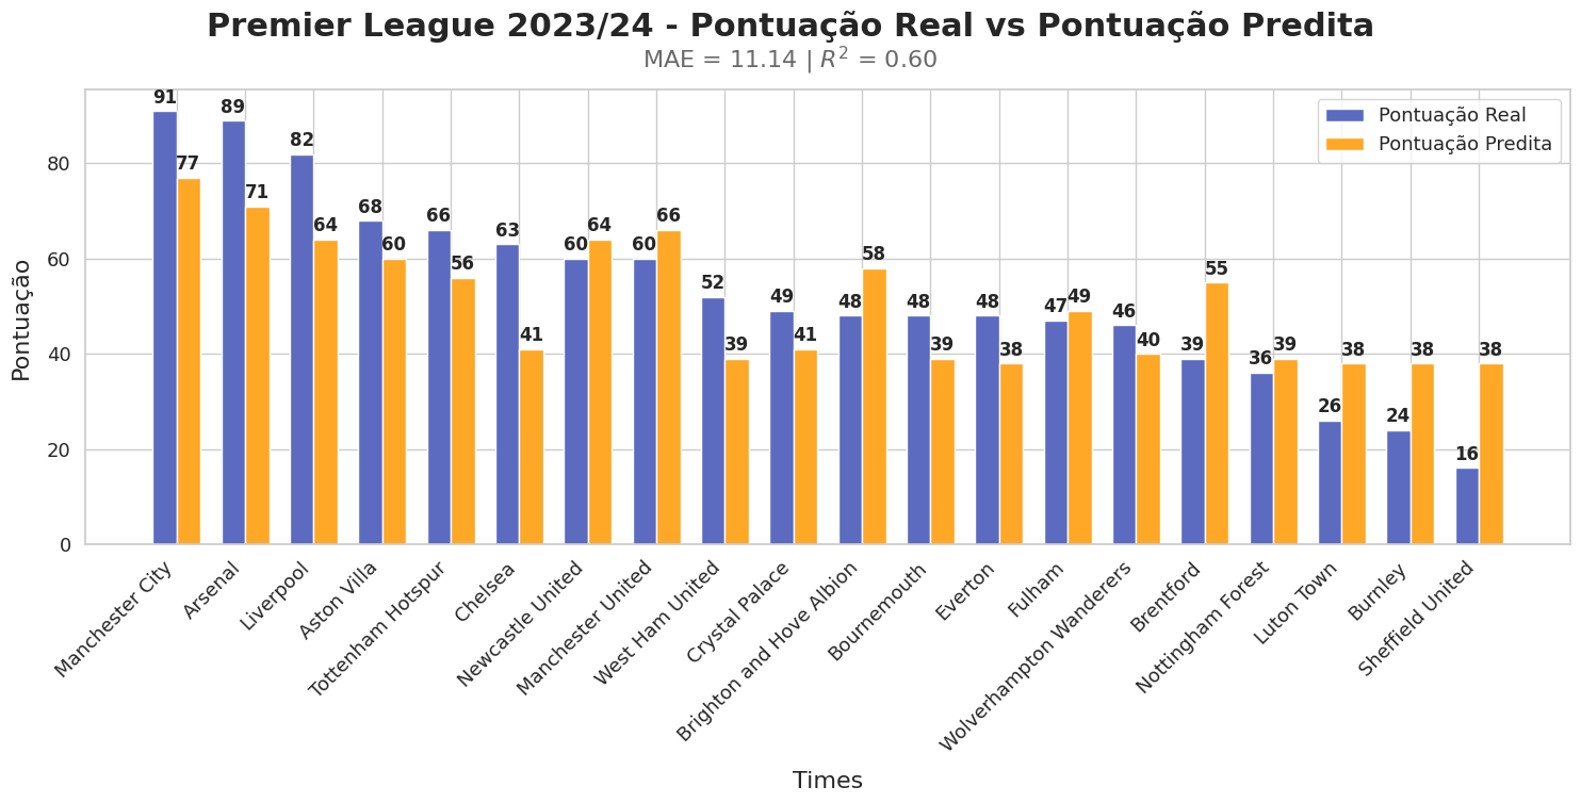
\includegraphics[width=1.3\textwidth]{imagens/pl_points.jpg}
    }
    \caption{Relação entre pontuações reais e previstas pelo modelo MLP na Premier League.}
    \label{fig:pl_points}
\end{figure}

Os resultados apresentados na Figura~\ref{fig:pl_points} indicam que o modelo MLP apresenta maior precisão ao estimar as pontuações de clubes que terminaram a 
temporada com valores próximos da média da liga. Times posicionados no centro da distribuição como Fulham, Manchester United e Newcastle United tendem a 
ter suas pontuações previstas com menor erro, comportamento comum em modelos preditivos sob alta incerteza: quando os atributos disponíveis não capturam 
toda a variabilidade do fenômeno, as previsões convergem naturalmente para valores intermediários. Esse resultado alinha-se com a literatura clássica, 
segundo a qual modelos preditivos em ambientes de alta variabilidade, como é o caso do futebol, tendem a gerar funções de saída menos
extremas e com menor amplitude, aproximando-se de valores centrais, devido a mecanismos de \textit{shrinkage} e ao balanço entre viéses e variância discutidos 
por Bishop~\cite{bishop2006}. Esse comportamento é análogo ao fenômeno estatístico conhecido como regressão à média.

Dessa forma, observa-se que o modelo MLP é capaz de capturar tendências gerais de desempenho dos clubes com base nas estatísticas individuais de seus jogadores, 
porém nota-se uma subestimação sistemática das equipes de desempenho elevado, como Manchester City, Arsenal e Liverpool, e uma superestimação das equipes de 
baixo desempenho, como Sheffield United, Burnley e Luton Town.

Com base nos resultados apresentados neste capítulo, foi possível identificar o modelo de AM que apresentou o melhor desempenho na tarefa de predição da pontuação 
final das equipes. A partir dessa definição, o modelo selecionado (MLP) passa a ser utilizado como função objetivo na etapa de otimização da composição de elencos. 
Dessa forma, no próximo capítulo são apresentados os procedimentos de PO empregados para simular contratações e avaliar configurações de elenco capazes de 
maximizar o desempenho previsto das equipes.